\chapter{Четвертий клас}

\problem
Розділи торти порівну на всіх запрошених:
\begin{enumerate}
    \item 6~тортів на 48~гостей;
    \item 8~тортів на 48~гостей;
    \item 9~тортів на 108~гостей;
    \item 15~тортів на 120~гостей.
\end{enumerate}

\begin{figure}[h]
    \centering
    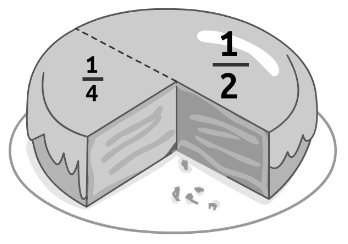
\includegraphics[width=0.3\textwidth]{4-01-1}
\end{figure}


\problem
У~кожного учня в~БеркоШко є: зошити в~клітинку~--- з~математики,
з~живого світу і~два зошити з~англійської, зошити в~лінійку~---
з~російської та української мови, а~також альбоми з~музики і~дослідів.
Скільки зошитів у~всіх учнів БеркоШко разом?


\problem
Валя замовила футболки для Варі, Макса, Росави~--- бо їм не~дісталося навесні,
а~також для Федька, Машки і~Сашка, бо вони свої за літо зносили або загубили :).
За всі футболки разом вона заплатила 696~грн.
Скільки коштує друк однієї футболки? 


\problem
Бабуся в’язала шкарпетки бійцям добровольчого батальйону.
Спершу плела з~синіх ниток, а~коли сині закінчилися, почала плести коричневі.
За два тижні вона встигла сплести 14~пар шкарпеток.
\begin{enumerate}
    \item З~якою швидкістю бабуся в’яже шкарпетки? 
    \item Скільки шкарпеток (скільки штук) синього кольору сплела бабуся,
    якщо вона помітила, що коричневих вийшла рівно четвертинка.
\end{enumerate}


\problem
Визнач відстані:

\begin{figure}[h]
    \centering
    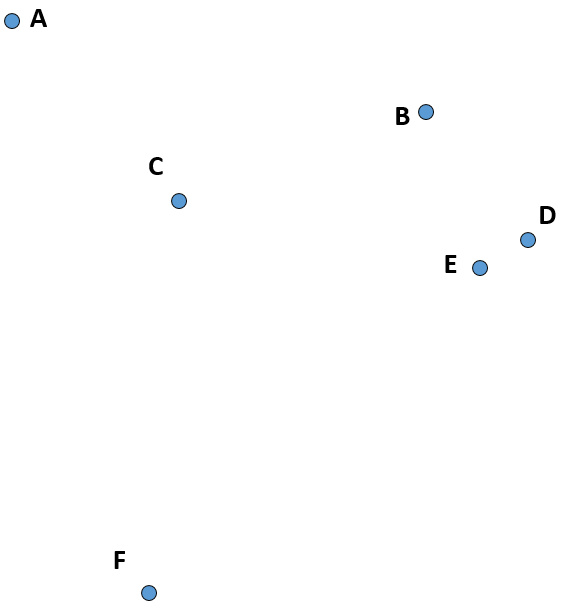
\includegraphics[width=0.6\textwidth]{4-05-1}
\end{figure}

\begin{tabular}{|c|c|c|}
    \hline
    Відрізок & Приблизно, см & Точно, см \\ \hline
    BC & & \\ \hline
    AE & & \\ \hline
    ED & & \\ \hline
    AF & & \\ \hline
    EF & & \\ \hline
    FD & & \\ \hline
\end{tabular}


\problem
% TODO: meaning of the problem?
Запиши скорочену умову~--- лише те, що необхідне для розв’язання,
зазнач одиниці вимірювання величин у~дужках, пояснення до кожної дії
і~відповідь.

Першою країною, яка почала досліджувати космос, був Радянський союз (СРСР),
на~той час Україна була в~його складі. Потім активно долучилися США.
Зараз космічні дослідження переважно міжнародні.

Трохи історії перших років космонавтики:
У~1957~році в~космос запустили перший супутник «Спутник-1» (СРСР).
Перша тварина у~космічному просторі~--- собака Лайка на «Спутник-2»
у~1957 році (СРСР).
Першим космонавтом став Юрій Гагарін у~1961~році (СРСР).
Вперше до Місяця долетів корабель «Луна-2» (без людей) у~1959 році,
а~в~1970~році на Місяць доставили перший автоматичний планетохід —
«Луноход-1» (СРСР).
Вперше у~відкритий космос вийшов Олексій Леонов у~1965 році (СРСР).
Першою людиною, що висадилася на Місяць став Ніл Армстронг у~1969~році (США).
Далі були польоти до інших планет і~орбітальні станції,
кому цікаво~--- можете почитати детальніше.

Перший український космонавт часів незалежності України~--- Леонід Каденюк.
У~1997~році він літав у~космос у~складі міжнародної команди корабля «Колумбія».
Його завданням було дослідження впливу невагомості на розвиток рослин:
ріпи, сої та моху. Політ тривав 16~днів. У~нього було по 12~рослин кожного виду.
Щодня він обстежував рослини і~результати досліджень записував у~протокол,
про кожну рослинку~--- на 1~сторінку. Наприкінці польоту Леонід Каденюк
написав звіт про вплив невагомості на рослини, який мав 3~розділи.
Перший розділ~--- вступ~--- мав 37~сторінок. Другий розділ містив всі
протоколи досліджень. А~в~третьому розділі були описані висновки~---
на 16~сторінках.
(Насправді, я не~знаю, скільки саме сторінок було у~звіті Леоніда Каденюка,
але сам космонавт, його політ і~дослідження рослин~--- точно були \smiley)


\problem
Виріши рівняння:
\begin{multicols}{2}
    \begin{enumerate}
        \item $4096 = 6194 - x$
        \item $678 - 3x = 597$
        \item $87 - x = x + 37$
        \item $2x + 66 = 117 - x$
        \item $831 - 3x = x + 391$
    \end{enumerate}
\end{multicols}


\problem
\problemname{Задача про авантюриста Джека}

\begin{quote}
\itshape
    -- А~хто такий авантюрист? \\
    -- Слово походить від французького «aventure»~--- «пригода».
    Але це не будь-яка пригода.
    В~українській і~російській мові слово набуло певного відтінку\ldots
    Зараз зрозумієте.
\end{quote}

Жив собі Джек. І~якось йому спало на думку вирушити на розшуки скарбів,
але у~нього не~було ні~карти, ні~команди, нічого. Тоді він позичив
у~сусідів 20~піастрів і~вирушив у~порт, найматися на корабель.

\begin{wrapfigure}{l}{0.4\textwidth}
    \begin{center}
        
\includegraphics[width=0.4\textwidth]{4-08-1}
    \end{center}
\end{wrapfigure}

Як і~всім авантюристам, на початку йому дуже щастило.
У~портовому кабаку він познайомився з капітаном, який саме шукав
матросів на корабель. Подейкували, що саме для пошуку скарбів.
Капітан спершу не хотів брати Джека, але той віддав йому всі свої
гроші і~сказав, що працюватиме просто за харчі, аби його тільки взяли.

Так корабель із капітаном і дванадцятьма матросами, одним з~яких був Джек,
вирушив на пошуки. У~капітана справді знайшлася карта закопаних скарбів,
а ще він виявився чесною людиною і~запропонував розділити знахідку по-чесному:
всім матросам однакові долі, а~капітанові~--- вдвічі більше, бо карта його.
Всі з цим погодились.

4~роки корабель шукачів нишпорив морями та океанами у~пошуках острова
скарбів і~зрештою таки знайшов. Велику скриню, в~якій виявилося
2340 золотих піастрів.

Їх розділили: капітанові~--- 2~долі, 12~матросам~--- по одній:

Ті монети, що не~змогли поділити, кинули в~море~--- на знак вдячності
за сприятливий вітер. І~вся команда вирішила пливти далі у~пошуках пригод,
але Джекові вже дуже кортіло додому. Тому він попрощався, забрав свою
частку скарбу і~зійшов у~найближчому порту. Повертатися додому йому було
через півсвіту, але пощастило домовитися з~кораблем, що вирушав у~його
рідні краї, за 10~піастрів.

Плив Джек дуже довго, майже рік, бо саме настав сезон штормів.
Втім таки дістався додому.

Першим ділом він пішов до сусіда віддати борг.

А~той розказав Джекові, що вирушаючи в~подорож, Джек забув заплатити
ренту за будинок і~всі ці 5~років банк нараховував йому борг.

Спантеличений Джек пішов у~банк, де йому виписали квитанцію на 150~піастрів,
які він мав сплатити негайно, аби не потрапити у~боргову яму.

Джек порахував гроші і~зажурився. Довелося знову позичати у~сусіда.

А~ввечері Джек сидів на ґанку свого будинку і~мріяв про те,
яким би мав бути той скарб, щоб йому не довелося знову залазити в~борги\ldots

\begin{quote}
    \itshape
    -- Так от, авантюрист може віддати 5~років свого життя
    на розшуки скарбів, лишившися по тому ні з~чим \smiley
\end{quote}


\problem
Намалюй положення стрілок за підказками:
\begin{enumerate}
    \item пів на восьму;
    \item 09:15;
    \item за чверть п’ята;
    \item 16:55;
    \item двадцять хвилин по дев’ятій;
    \item двадцять хвилин на дев’яту;
    \item перша;
    \item за 25 хвилин десята.
\end{enumerate}

\begin{figure}[h]
    \centering
    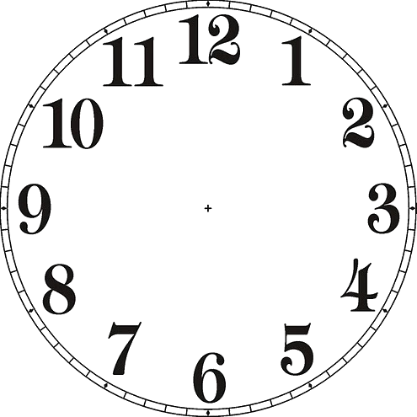
\includegraphics[width=0.3\textwidth]{4-09-1}
\end{figure}


\problem
На Берківці потрібно було замовити дрова.
У~кожну з~5~хаток П'ятихаток і~ще у~Рогатий дім потрібно по 4~куб.~м дрів,
а~в~школу~--- 6~куб.~м.
У~самоскид вміщається 6~куб.~м, які коштують 2800~грн.

Скільки машин дрів необхідно замовити? Скільки це коштуватиме? 
Як розподілити дрова між усіма хатками порівну?

\begin{figure}[h]
    \centering
    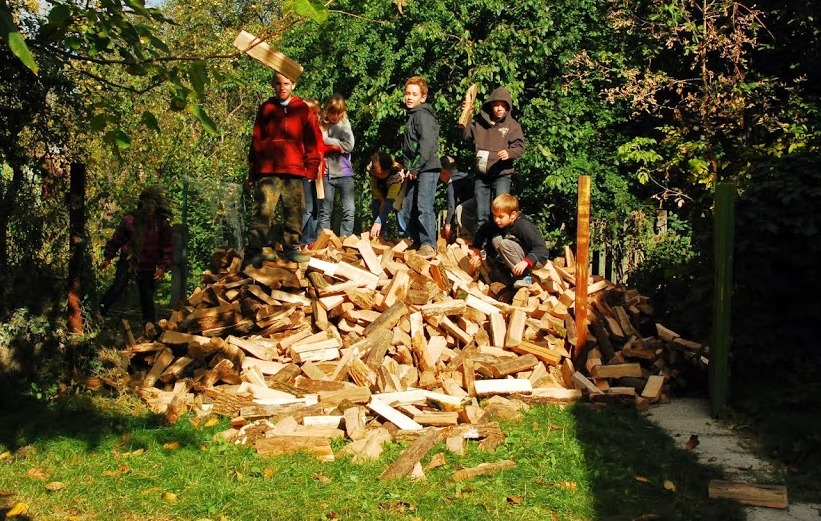
\includegraphics[width=0.8\textwidth]{4-10-1}
\end{figure}

Коли привезли першу машину, самоскид скинув дрова на купу і~5~людей
складало дрова в дровітниці. Їм знадобилося 3~години.
Скільки часу знадобиться 3~людям, щоб розкласти таку саму кількість дрів?
А~якщо комусь доведеться працювати насамоті, скільки часу він складатиме дрова?


\problem
Дізнайся довжини мостів в~Києві: Московського, Патона,
Паркового («Мосту закоханих») в Маріїнському парку, Залізничного мосту.
Визнач найдовший, найкоротший.
Якщо довжина тролейбуса 18~м, то скільки таких тролейбусів
вміститься на кожному мосту, впритул один за одним?


\problem
Тома прочитала цікаву книжку за 15~днів. У~книжці було 315~сторінок.
Потім цю книжку попросила почитати Іванка. Їй книга так сподобалася,
що вона читала кожного дня на 7~сторінок більше, ніж Тома.
Через скільки днів Іванка зможе повернути Томі книжку?


\problem
Виріши нерівності:
\begin{multicols}{2}
    \begin{enumerate}
        \item $9000 : a > 450$
        \item $11 \cdot x > 1870$
        \item $4 \cdot y - 8 <= 100$
        \item $5 \cdot (k + 17) >= 175$
    \end{enumerate}
\end{multicols}


\problem
Підрахуй, скільки хлібу з’їдає твоя родина за тиждень.
Якого розміру поле мала обробити родина, щоб мати хліб на весь рік?
(У середньому родина з~чотирьох осіб~--- тато, мама і~двоє діток~---
з’їдає 4~хлібини на тиждень. Вважаємо, що 1~хлібина важить 1~кг,
а~борошна на неї потрібно 400~г. Вихід борошна із зерна~--- 4/5 його ваги.
А~на одному гектарі вирощують від 10 до 150 центнерів пшениці,
залежно від врожайності ґрунтів і~сприятливості умов.
Приймаємо середній показник по Україні за часів СРСР~---
40~центнерів з~1~гектара.)


\problem
Том Сойєр сам міг би пофарбувати паркан за 6~годин,
а~Гекльберрі Фінн~--- за 3~години. Але вони почали фарбувати його вдвох,
одночасно, з~протилежний кінців, назустріч один одному.
Через який час вони зустрінуться, пофарбувавши весь паркан,
довжина якого 120~м?


\problem
Зустрілись у~прерії два ковбої Том і~Джері. Постояли, побалакали та й
роз’їхалися кожний на своє ранчо. Том поїхав зі швидкістю $v$ на схід,
а~Джері, зі швидкістю на $x$ більшою~--- на захід. Їхали до своїх ранчо
вони однаковий час $t$. Яка відстань між ранчо Тома і~Джері?

А~тепер обчисли відстань, якщо швидкість Тома 47~м/хв,
у~Джері~--- на 4~м/хв більше, а~роз’їжджалися вони 2~години?


\problem
Відстань між містом Бурмосиків і~містом Викрутасиків~--- 204~км.
Викрутасики добігають у~гості до Бурмосиків за 6~годин.
За скільки годин доходять у~гості Бурмосики,
якщо їхня швидкість на 22~км/год менша, ніж швидкість Викрутасиків?


\problem
\problemname{Незавершена мандрівка}
Троє хлопців з~містечка Радомишль, що на річці Тетерів, зробили пліт.
І~зібралися вирушити на ньому в~мандри до моря. Запаслися харчами,
теплим одягом, картою, різним інструментом і о~9~ранку відпливли вниз
за течією. Вже опівдні вони пропливли повз село Березці, в якому жила
бабуся одного з~хлопців, а~він знав, що до того села відстань 6~км.
Отже вони могли дізнатися, з~якою швидкістю вони сплавляються,
і~розрахувати, коли дістануться до моря.

\begin{wrapfigure}{r}{0.4\textwidth}
    \begin{center}
        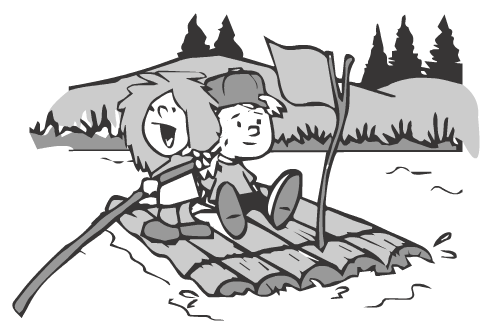
\includegraphics[width=0.4\textwidth]{4-18-1}
    \end{center}
\end{wrapfigure}

Але не все так сталось, як гадалось. Цього дня тато одного з~хлопців
о~9:00 відплив на своєму катері вверх по течії. Катер був доволі швидкий,
минулого літа на озері він розганявся до 14~км/год.

І~ось, коли відстань між ними (катером і~плотом) становила вже 84~км,
тато зрозумів, що хлопці попливли в~мандри і~до вечері додому не встигнуть.
Розвернувся і~поплив їх наздоганяти.

Скільки часу минуло з~відчалювання у~Радомишлі до того, як тато
розвернув човна і~поплив навздогін хлопцям?
Скільки часу він їх наздоганятиме?
Яку відстань встигнуть пропливти хлопці на плоті, поки тато їх не перехопить?


\problem
Прямокутний лист фанери довжиною 5~дм і~шириною 3~дм розпиляли на квадратики
зі стороною 1~см.
Скільки таких квадратиків вийшло?


\problem
Збираючися в~похід, Макс купив собі новий тент і~для міцності вирішив
обшити його тасьмою. Ширина тенту~--- 6~м, а довжина~--- на 4~м більша.
Скільки метрів тасьми йому знадобиться для цього?


\problem
Вовк пробіг певну відстань за якийсь час.
Лось чверть цього шляху пробіг за час, вдвічі менший.
На скільки швидкість лося менша за швидкість вовка?


\problem
За прогнозом погоди від 1~січня 2015~року температура повітря вдень
у~Києві складатиме:

\begin{multicols}{2}
    7~січня~--- 0~градусів

    8~січня~--- 0~градусів

    9~січня~--- 0~градусів

    10~січня~--- 2~градуси

    11~січня~--- 3~градуси

    12~січня~--- 4~градуси

    13~січня~--- 3~градуси

    14~січня~--- 2~градуси

    15~січня~--- 2~градуси

    16~січня~--- 4~градуси
\end{multicols}

Яку середню температуру повітря очікують у~Києві з~7 до 16~січня?


\problem
Виріши рівняння:
\begin{multicols}{2}
    \begin{enumerate}
        \item $x : 100 = 0$
        \item $x + 100 = 100$
        \item $x \cdot 100 = 100\,000$
        \item $x - 100 = 100\,000$
    \end{enumerate}
\end{multicols}


\problem
Обчисли:
\begin{enumerate}
    \item $1530 : (12 \cdot 6 - 38) \cdot 15$
    \item $4840 + 12\,903 - 80\,125 : 5$
    \item $(420 \cdot 20 - 210 \cdot 30) : 100 \cdot (600 - 591)$
    \item $(500 \cdot 10 - 500 : 10) \cdot 6 : (1000 - 997)$
\end{enumerate}


\problem
Щомісяця батьки дають хлопчикові 100~грн, з~них 65~грн він витрачає
на проїзд і~смаколики, а~решту відкладає на придбання моделей літачків.
Через який час він назбирає достатньо грошей, щоб придбати 50~моделей літачків,
кожний з~яких коштує 28~грн?


\problem
Жіночка продає в~метро календарі.
Закупає у~видавництві 12~календарів за 50~грн, а~продає кожний по 5~грн.
Скільки вона заробить, якщо продасть 30~календарів?


\problem
Черепашка з~дитинства мріяла подорожувати. І~ось одного сонячного ранку
вона поклала в~наплечник GPS-навігатор, щоб не заблукати,
і~вирушила в~мандрівку.

Першого дня вона доповзла до лісу і~влаштувалася на ночівлю під крислатим
дубом. Перед сном черепашка визначила за навігатором, що цього дня
проповзла рівно 2645~м.

Другого дня вона мандрувала лісом, шаруділа листям, милувалася сонячними
променями, які пробивалися крізь гілля, ласувала ожиною і~суницями.
І~ввечері знову перевірила за навігатором, яку~ж відстань подолала.
Виявилося, що за другий день вона проповзла рівно стільки~ж,
скільки й за перший.

Третього дня їй вдалося доповзти до гарного лісового озера,
вона влаштувалася на крутому беріжку і~спробувала визначити,
яку відстань вона проповзла, але в~навігаторі щось заглючило
і~він не~показував відстані.

Черепашка засмутилась і~почала натискати на всі кнопочки меню врізнобій,
аж~раптом навігатор видав повідомлення, що за третій день вона проповзла
на 1740~м менше, ніж за попередні два дні разом.

То як далеко від дому відповзла черепашка?


\problem
Підприємець придбав 18~дюжин стільців по 3000~грн за дюжину.
За перевезення заплатив 800~грн.
Відтак кожний стілець продав за 300~грн.
Скільки він заробив?


\problem
У~коробці 80~сірників, коштує вона 1~грн.
Скільки коштують 2000~сірників?


\problem
Перед тим, як їхати з~БеркоШко на музику, Клим і~Макс сіли перекусити курагою.
Макс з’їв вдвічі більше за Клима, а~Клим на 6~куражинок менше за Макса.
Скільки кураги з’їв Клим?


\problem
На яке число треба поділити 22849, щоб вийшло 36 і~ще 25 в~остачі?


\problem
По дорозі до школи Клим відшукує воронячі гнізда. Вже нарахував 21~гніздо.
Навесні в~кожному з~них з’явиться в~середньому по 3~вороненятка.
Цікаво, скільки вороненят народиться тут за 5~років?


\problem
Чи можна намалювати хатку, на відриваючи олівця від паперу і~на проводячи
жодну лінію двічі?
З~якої точки варто починати?

\begin{figure}[h]
    \centering
    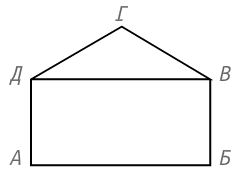
\includegraphics[width=0.3\textwidth]{4-33-1}
\end{figure}


\problem
На Великому Пагорбі на сторожі сиділи двоє індіанців:
Орлине Око з~племені ірокезів і~Вертлявий Тхір з~племені делаварів.

Раптом вони помітили на узліссі блідошкірих, які шикувалися для нападу.
Кожний з~індіанців побіг попередити своє плем’я.
Табори обох племен розташовані на однаковій відстані від Великого Пагорба~---
5~кілометрів, але делавари дізналися про напад блідолицих через 20~хвилин,
а~ірокези~--- через 30~хвилин.

На скільки Вертлявий Тхір бігає швидше за Орлине Око?


\problem
Збільши у~68~разів частку суми чисел 4893 і~1527 та числа 30.


\problem
Два потяги одночасно виїхали назустріч одне одному.
Швидкість одного 80~км/год, а~другого~--- 7/8 від швидкості першого потяга.
Через 2~години після початку руху їм залишалося проїхати
1/3 початкової відстані.
Скільки кілометрів становила відстань між потягами на початку?


\problem
Який середній вік людей, які перебувають у~БеркоШко просто зараз?


\problem
% TODO: meaning of problem?
Одного дня беркошколярики прийшли до школи як завжди о~9:15.
Знайшли на поличці пісочний годинник на 15 хвилин і~почали відміряти ним час.
Щойно пісок пересипався з~однієї чаші годинника в~іншу,
його знову перевертали, навіть під час занять,
навіть під час великої перерви.
Впродовж дня діти встигли перевернути годинник 27~разів.
І~коли пісок пересипався востаннє, всі пішли додому.
О~котрій годині всі пішли додому того дня?


\problem
Для розписування писанок перед Великоднем Женя попросила всіх понавидувати
вдома яєць і~принести до БеркоШко. Коли всі діти поскладали принесені яйця
в~лоточки, вдалося заповнити 4~лотки на десяток яєць і~2~--- на~18.
Ще один лоток на 15~яєць принесла з~собою Женя.
Діти старанно робили писанки, топили віск, обережно малювали писачками,
але декілька яєць все~ж таки висковзнули з~рук і~розбилися.
Коли діти закінчили заняття писанкарством, то нарахували 87~готових писанок.
То скільки яєць розбилося?


\problem
Якось Тома, Юля, Клим, Федько, Іванка, Варя, Маша і~Макс гралися
в~індіанців і~випадково знайшли поза школою моток ліски, довжиною 7~м 44~см.
І~вирішили зробити з~неї тятиву для своїх луків.
Як розділити ліску на всіх порівну і~якої довжини тятива вийде у~кожного?
